
%(BEGIN_QUESTION)
% Copyright 2015, Tony R. Kuphaldt, released under the Creative Commons Attribution License (v 1.0)
% This means you may do almost anything with this work of mine, so long as you give me proper credit

Tegn piler ved hver av de to magnetventilene som viser luftstrøm i energisert (E) og spenningsløs (D) tilstand, gitt at begge magnetventiler må ``trippe'' for å tvinge prosessventilen til fail-posisjon (2oo2 for trip):

$$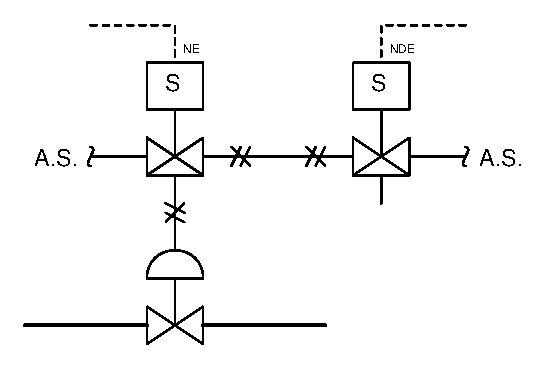
\includegraphics[width=15.5cm]{i00982x01.eps}$$

\underbar{file i00982}
%(END_QUESTION)





%(BEGIN_ANSWER)

$$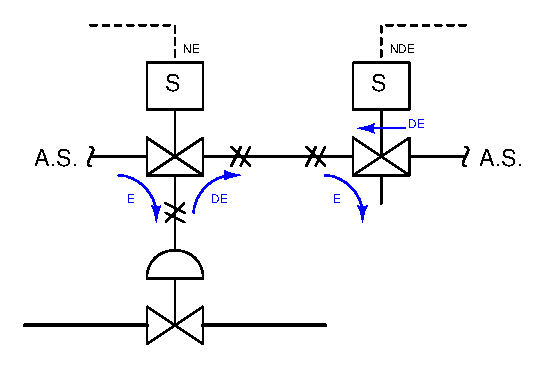
\includegraphics[width=15.5cm]{i00982x02.eps}$$
 
%(END_ANSWER)





%(BEGIN_NOTES)


%INDEX% Final Control Elements, valve: fail-safe solenoids
%INDEX% Process: incinerator (realistic P&ID shown)

%(END_NOTES)

